\documentclass{fisattraining}
\title{Internship report}
\team{Roby Jacob}
\author{Roby Jacob}
\begin{document}
\maketitle
\makecert

\newpage
\pagenumbering{roman}
\setcounter{page}{1}
\newgeometry{top=4cm,bottom=0.1cm}
\thispagestyle{plain}
\renewcommand\abstractname{Company Profile}
\begin{abstract}
\vspace{5cm}
Lorem ipsum dolor sit amet, consectetur adipiscing elit. Morbi urna mauris, sagittis sit amet aliquet ut, facilisis et nibh. Praesent turpis tortor, dignissim ut interdum eu, porttitor ut orci. Curabitur laoreet malesuada fermentum. In posuere, purus eu pulvinar luctus, eros urna tempor magna, eu tincidunt erat eros nec turpis. Vestibulum at semper lacus. Nullam tristique lacus vel nibh porta a vehicula tellus volutpat. Pellentesque cursus ullamcorper ante, ut eleifend nisl aliquam id. Nulla porta ornare fermentum. Aliquam id magna sed erat malesuada viverra. Donec non mauris eros, nec egestas ligula. Suspendisse eu tempor ligula. Aliquam egestas nulla vel augue iaculis iaculis nec in risus. Pellentesque habitant morbi tristique senectus et netus et malesuada fames ac turpis egestas. Praesent malesuada fringilla sapien a faucibus.
\end{abstract}


\newpage
\renewcommand\abstractname{ACKNOWLEDGMENT}
\thispagestyle{plain}
\begin{abstract}
\vspace{5cm}
I would like to express my special thanks of gratitude to my teachers
Reshmi.R and Jestin Joy as well as our principal Dr. George Issac who gave
me the permission to do this wonderful internship on the topic System Oriented Architecture for automotive,at FISAT under the guidance of Jestin Joy.They provide me with this program, which also helped me in doing a lot of Research and I came to know about so many new things,I am really thankful to them. Secondly
I would also like to thank my parents and friends who helped me a lot in
completing this project within the limited time frame.
\vspace{1cm}
\begin{flushright}
Roby Jacob
\end{flushright}
\end{abstract}
\newpage

\restoregeometry
\tableofcontents
\newpage

\cleardoublepage
\addcontentsline{toc}{chapter}{\listfigurename}
\listoffigures
\newpage

\chapter{Technology}
\pagenumbering{arabic}
\setcounter{page}{1}
\renewcommand{\baselinestretch}{1.50}
\section{Introduction}
Service Oriented Architecture(SOA) is a style of software design in which  services are provided through a communication protocol. A service is defined as a function that is  well-defined, self-contained,reusable and does not depend on any other service. SOA promotes loose coupling between the service, i.e each service need not know what the other service does, this makes it easy for developers to switch between service providers who provide the same services.
\begin{figure}[h!]
\begin{center}
\includegraphics[scale=.2]{mandelbrot}
\caption{SOA stages}
\end{center}
\end{figure}
The figure explains what are the different roles in a SOA system. The service providers may have several services implemented, information about these are  published in a service registry.The client(i.e. the service requestor) who wishes to use a service find the service details from the registry and locates the service provider. Then the client binds with the service provider and access the required service using a service id over a standard protocol(like TCP, UDP).
\section{Advantages}
The main advantages of SOA are\\
  1)Reusability: As services are self contained pieces, they can be used for different clients.\\
  2)Loose Coupling: Each functions are divided into services, these are not dependent on other services.\\
  3)Easier debugging: Since each service is self contained it is easy to test and debug features\\
  4)Platform independent

\section{SOA in automotive}
SOA is currently is not common in automotive mainly because of the Overhead of SOA i.e the high resource required and the testing required which did not have any added benefits. But with the increase of computational power in car and the development of self driving cars SOA can improve the experience of end user and also manufactures. The main advantages of using SOA will be the high flexibility which will allow change to be made during runtime and also services outside and inside the car can be linked. The main protocol developed for this is SOME/IP.\\
\textbf{SOME/IP}:\\
Scalable service-Oriented MiddlewarE over IP(SOME/IP) is an automotive middleware solution that can be used for control messages. It is the only middleware protocol integrated into AUTOSAR.\\
Let's start with the three main parts of the SOME/IP specification:
\begin{itemize}
\item On-wire format
\item Protocol
\item Service discovery
\end{itemize}
\textbf{SOME/IP On-Wire Format}\\
In principle, SOME/IP communication consists of messages sent between devices or subscribers over IP. Consider the following picture:
\begin{figure}[h!]
\begin{center}
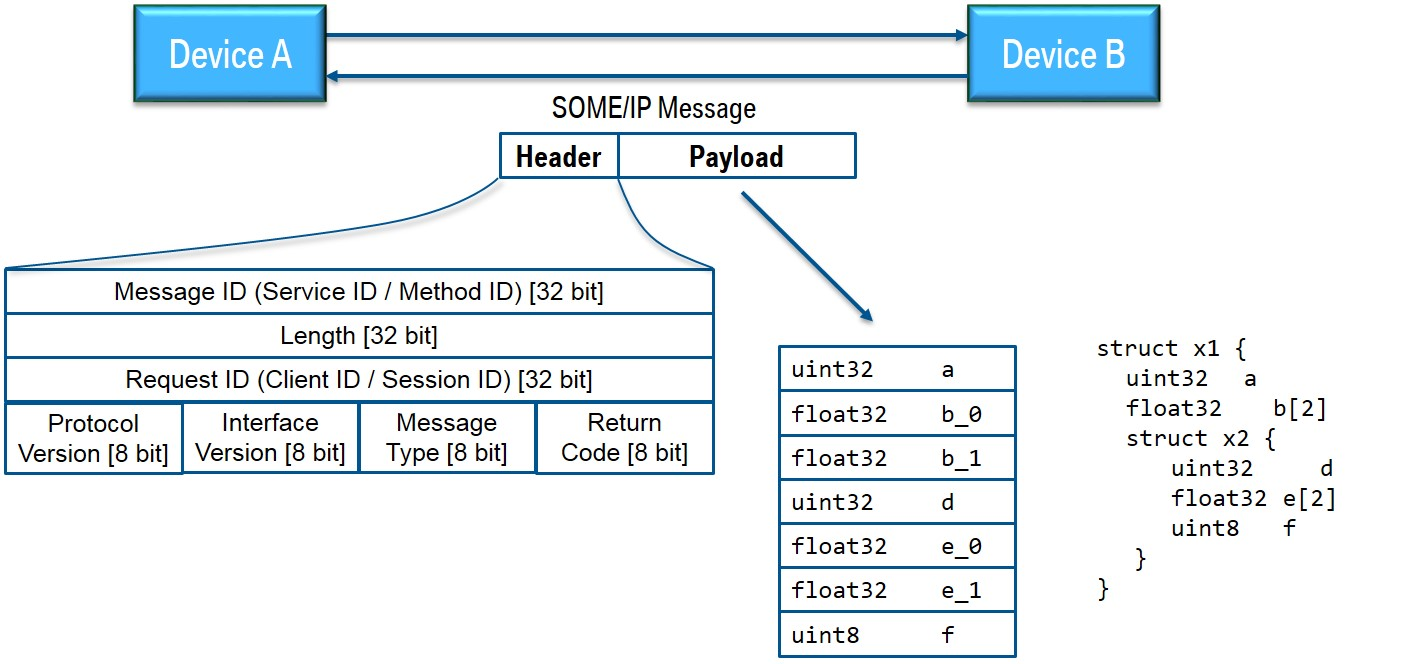
\includegraphics[scale=.5]{SOMEIPOnWireFormat}
\caption{vsome/ip packet format}
\end{center}
\end{figure}\\
\textbf{SOME/IP Protocol}\\
In this section mainly 2 points are important and shall be described now:
\begin{itemize}
\item the so-called transport bindings (UDP and TCP)
\item the basic communication patterns publish/subscribe and request/response.
\end{itemize}
As mentioned above the underlying transport protocol can be UDP or TCP. In the UDP case the SOME/IP messages are not fragmented; it can be that more than one message is in one UDP packet but one message cannot be longer than a UDP package can be (up to 1400 Bytes). Bigger messages must be transported via TCP. In this case all the robustness features of TCP are used. If a synchronization error in the TCP stream occurs, the SOME/IP specification allows so-call magic cookies in order to find again the beginning of the next message.\\
Please note that service interfaces must be instantiated and because there might be several instances of the same interface there must be an additional identifier for the instance defined (instance ID). However the instance ID is not part of the header of the SOME/IP message. The instance is identified via the port number of the transport protocol; that means that it is not possible that several instances of the same interface are offered on the same port.
Please take now a look at the following picture which shows the basic SOME/IP communication patterns:
\begin{figure}[h!]
\begin{center}
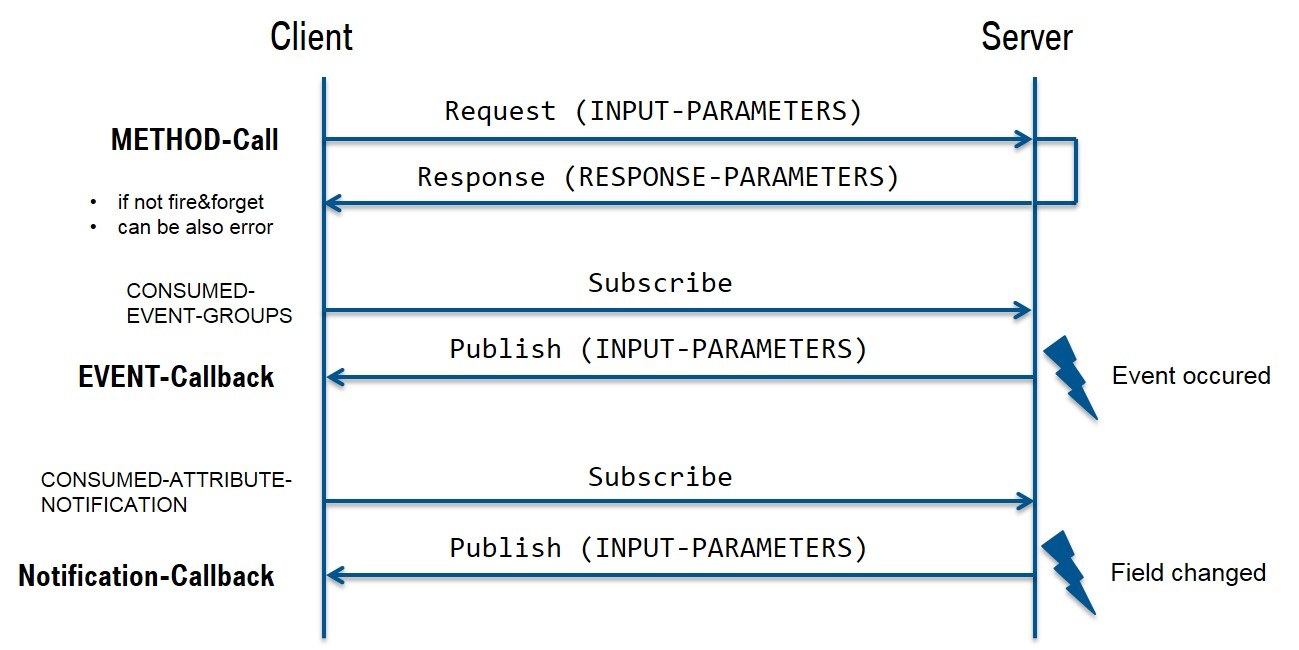
\includegraphics[scale=.5]{SOMEIPProtocol}
\caption{SOME/IP communication patterns}
\end{center}
\end{figure}
In addition to the standard REQUEST/RESPONSE mechanism for remote procedure calls there is also the PUBLISH/SUBSCRIBE pattern for events. Note that events in the SOME/IP protocol are always grouped in an event group; therefore it is only possible to subscribe to event groups and not to the event itself. The SOME/IP specification also knows "fields"; in this case the setter/getter methods are following the REQUEST/RESPONSE pattern and notfication messages of changes are events. The subscription itself is done via the SOME/IP service discovery.\\
\textbf{SOME/IP Service discovery}\\
The SOME/IP Service Discovery is used to locate service instances and to detect if service instances are running as well as implementing the Publish/Subscribe handling. This is mainly done via so-called offer messages; that means that each device broadcasts (multicasts) messages which contain all the services which are offered by this device. SOME/IP SD messages are sent via UDP. If services are required by client applications but at the moment not offered, then also "find messages" can be sent. Other SOME/IP SD messages can be used for publishing or subscribing an eventgroup.\\
The following picture shows the general structure of a SOME/IP SD message.
\begin{figure}[h!]
\begin{center}
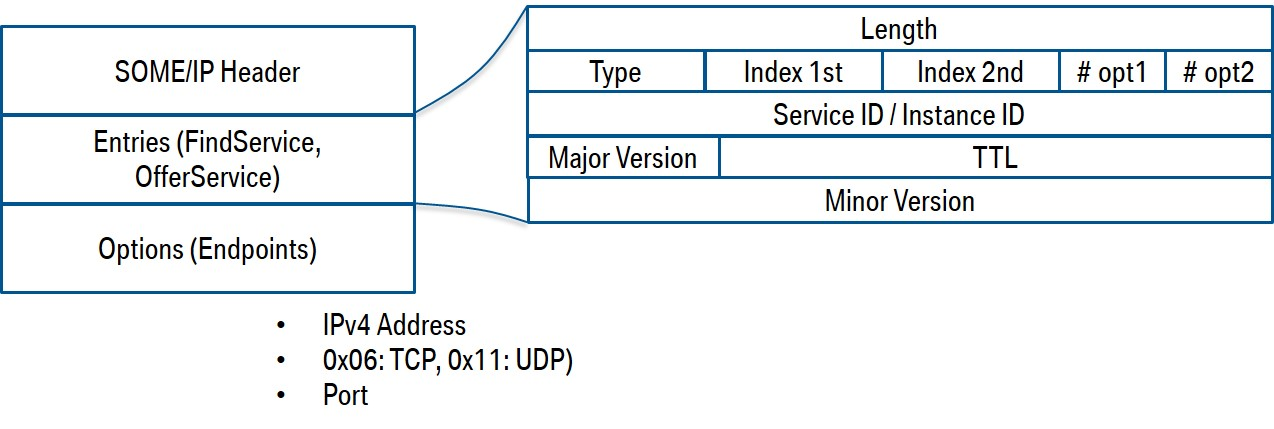
\includegraphics[scale=.5]{SOMEIPServiceDiscovery}
\caption{SOME/IP service discovery message}
\end{center}
\end{figure}
\section{VSOME/IP}
VSOME/IP is GENIVI's implementation of SOME/IP.\\
\textbf{Short overview}\\
Let's have a short look to the basic structure of the GENIVI implementation of SOME/IP which is called vsomeip.
\begin{figure}[h!]
\begin{center}
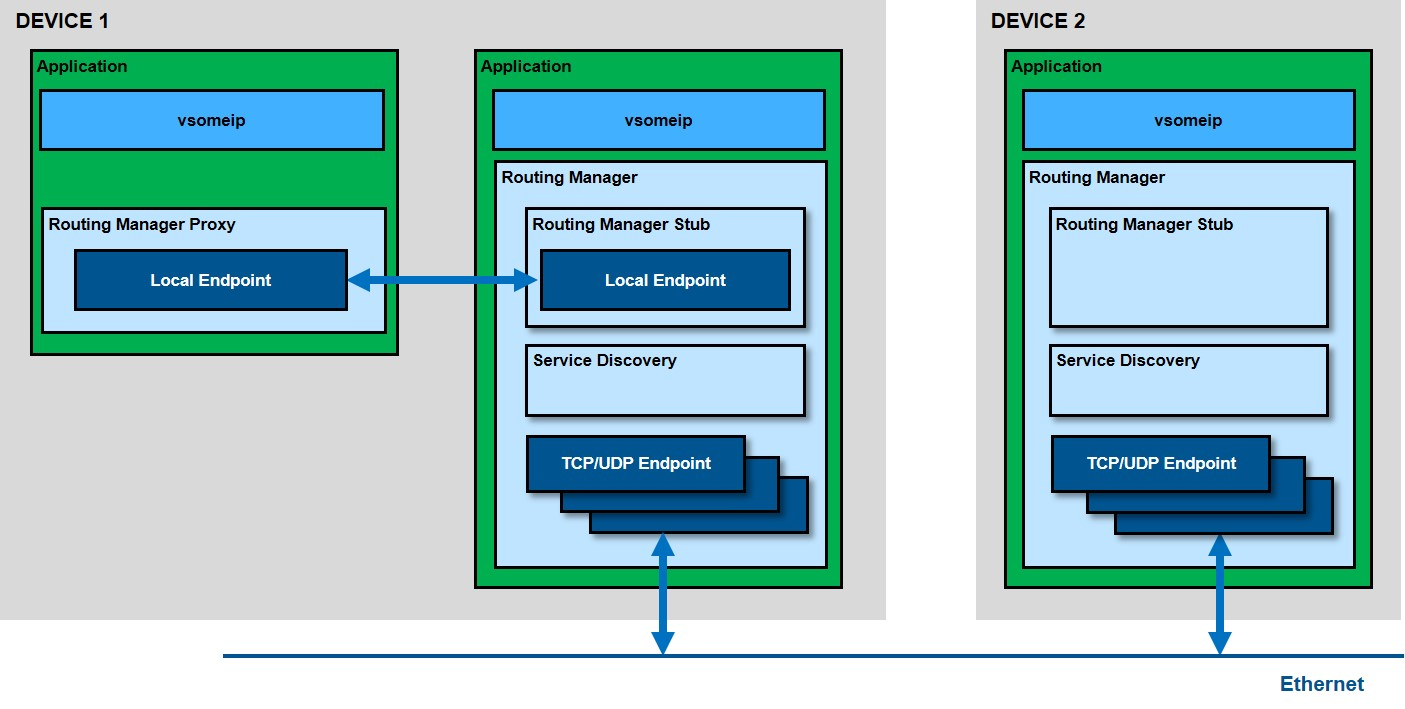
\includegraphics[scale=.5]{vsomeipOverview}
\caption{vsomeip overview}
\end{center}
\end{figure}\\
As shown in the picture vsomeip covers not only the SOME/IP communication between devices (external communication) but also the internal inter process communication. Two devices communicate via so-called communication endpoints which determine the used transport protocol (TCP or UDP) and its parameters as the port number or other parameters. All these parameters are configuration parameters which can be set in a vsomeip configuration file (json file, see vsomeip user guide). The internal communication is done via local endpoints which are implemented by unix domain sockets using the Boost.Asio library. Since this internal communication is not routed via a central component (e.g. like the D-Bus daemon), it is very fast.\\
The central vsomeip routing manager gets messages only if they have to be sent to external devices and he distributes the messages coming from outside. There is only one routing manager per device; if nothing is configured the first running vsomeip application also starts the routing manager.
\chapter{Daily Diary}


\section{Day 1 (June 30 2018)}
Installed Qemu virtual machine
\section{Day 2 (July 2 2018)}
Build yocto image
\section{Day 3 (July 3 2018)}
Ran yocto image in Qemu
\section{Day 4 (July 4 2018)}
Ran multiple images on multiple Qemu instances
\section{Day 5 (July 5 2018)}
Communicate between Qemu instances
\section{Day 6 (July 6 2018)}
Learn some/ip
\section{Day 7 (July 7 2018)}
Analysed vsomeip code
\section{Day 8 (July 8 2018)}
Ran vsomeip example code
\section{Day 9 (July 9 2018)}
Communicate multiple client vs single service
\section{Day 10 (July 10 2018)}
Communicate multiple client vs multiple service
\section{Day 11 (July 11 2018)}
Sample set up for running it in IVI
\chapter{Summary}
Learnt SOA and how to implement it in automotive using vsomeip library

\end{document}

